\chapter{Software Architecture} \label{chap:software_details}

  \section {Use Case View}
    
    The developed application enables the user to create a detailed terrain from a deterministic base surface. To achieve this goal several features, that aid the user in this process, were implemented. This features are specified in Table \ref{table:user_stories} in the form of user stories. Given the nature of this application only one actor, called User, is needed.
    
    
    \begin{table}[h!]
  \centering
  \renewcommand{\arraystretch}{1.5}
  \begin{tabularx}{\linewidth}{|l|l|b|}
	\hline
    \textbf{Code} & \textbf{Name} & \textbf{Description} \\ \hline
    US-001 & Load Base Surface & As a User I want to load a surface from an image so that I can create a detailed version of it. \\ \hline
    US-002 & Export Result & As a User I want to export the result so that I can use it in other applications. \\ \hline
    US-003 & Add Detail & As a User I want to add detail to a previously loaded base surface. \\ \hline
    US-004 & See Result & As a User I want to see my result as I change the parameters so that I can adjust them more easily. \\ \hline
    US-005 & History & As a User I want to be able to consult a list of previously edited terrains so that I can track my work. \\ \hline
    US-006 & History Parameters & As a User I want to have access to the parameters used in previously edited terrains. \\ \hline
    
  \end{tabularx}
  
  \caption{User Stories}
  \label{table:user_stories}
\end{table}
    
    \subsection {User Interface}
    
      The application was developed using Google's material design \cite{Google2016} for the user interface style. The editor is the main page of the application and it is shown in Figure \ref{fig:editor_page}. It contains a menu bar (1) where the user has access to the available functions, a details panel (2), which has the parameter controllers, a list with the previously results (3), a panel where the details of the selected previous result are displayed (4) and a canvas where the preview of the current current terrain is rendered (5).
      
      \begin{figure}[H]
      	\centering
      	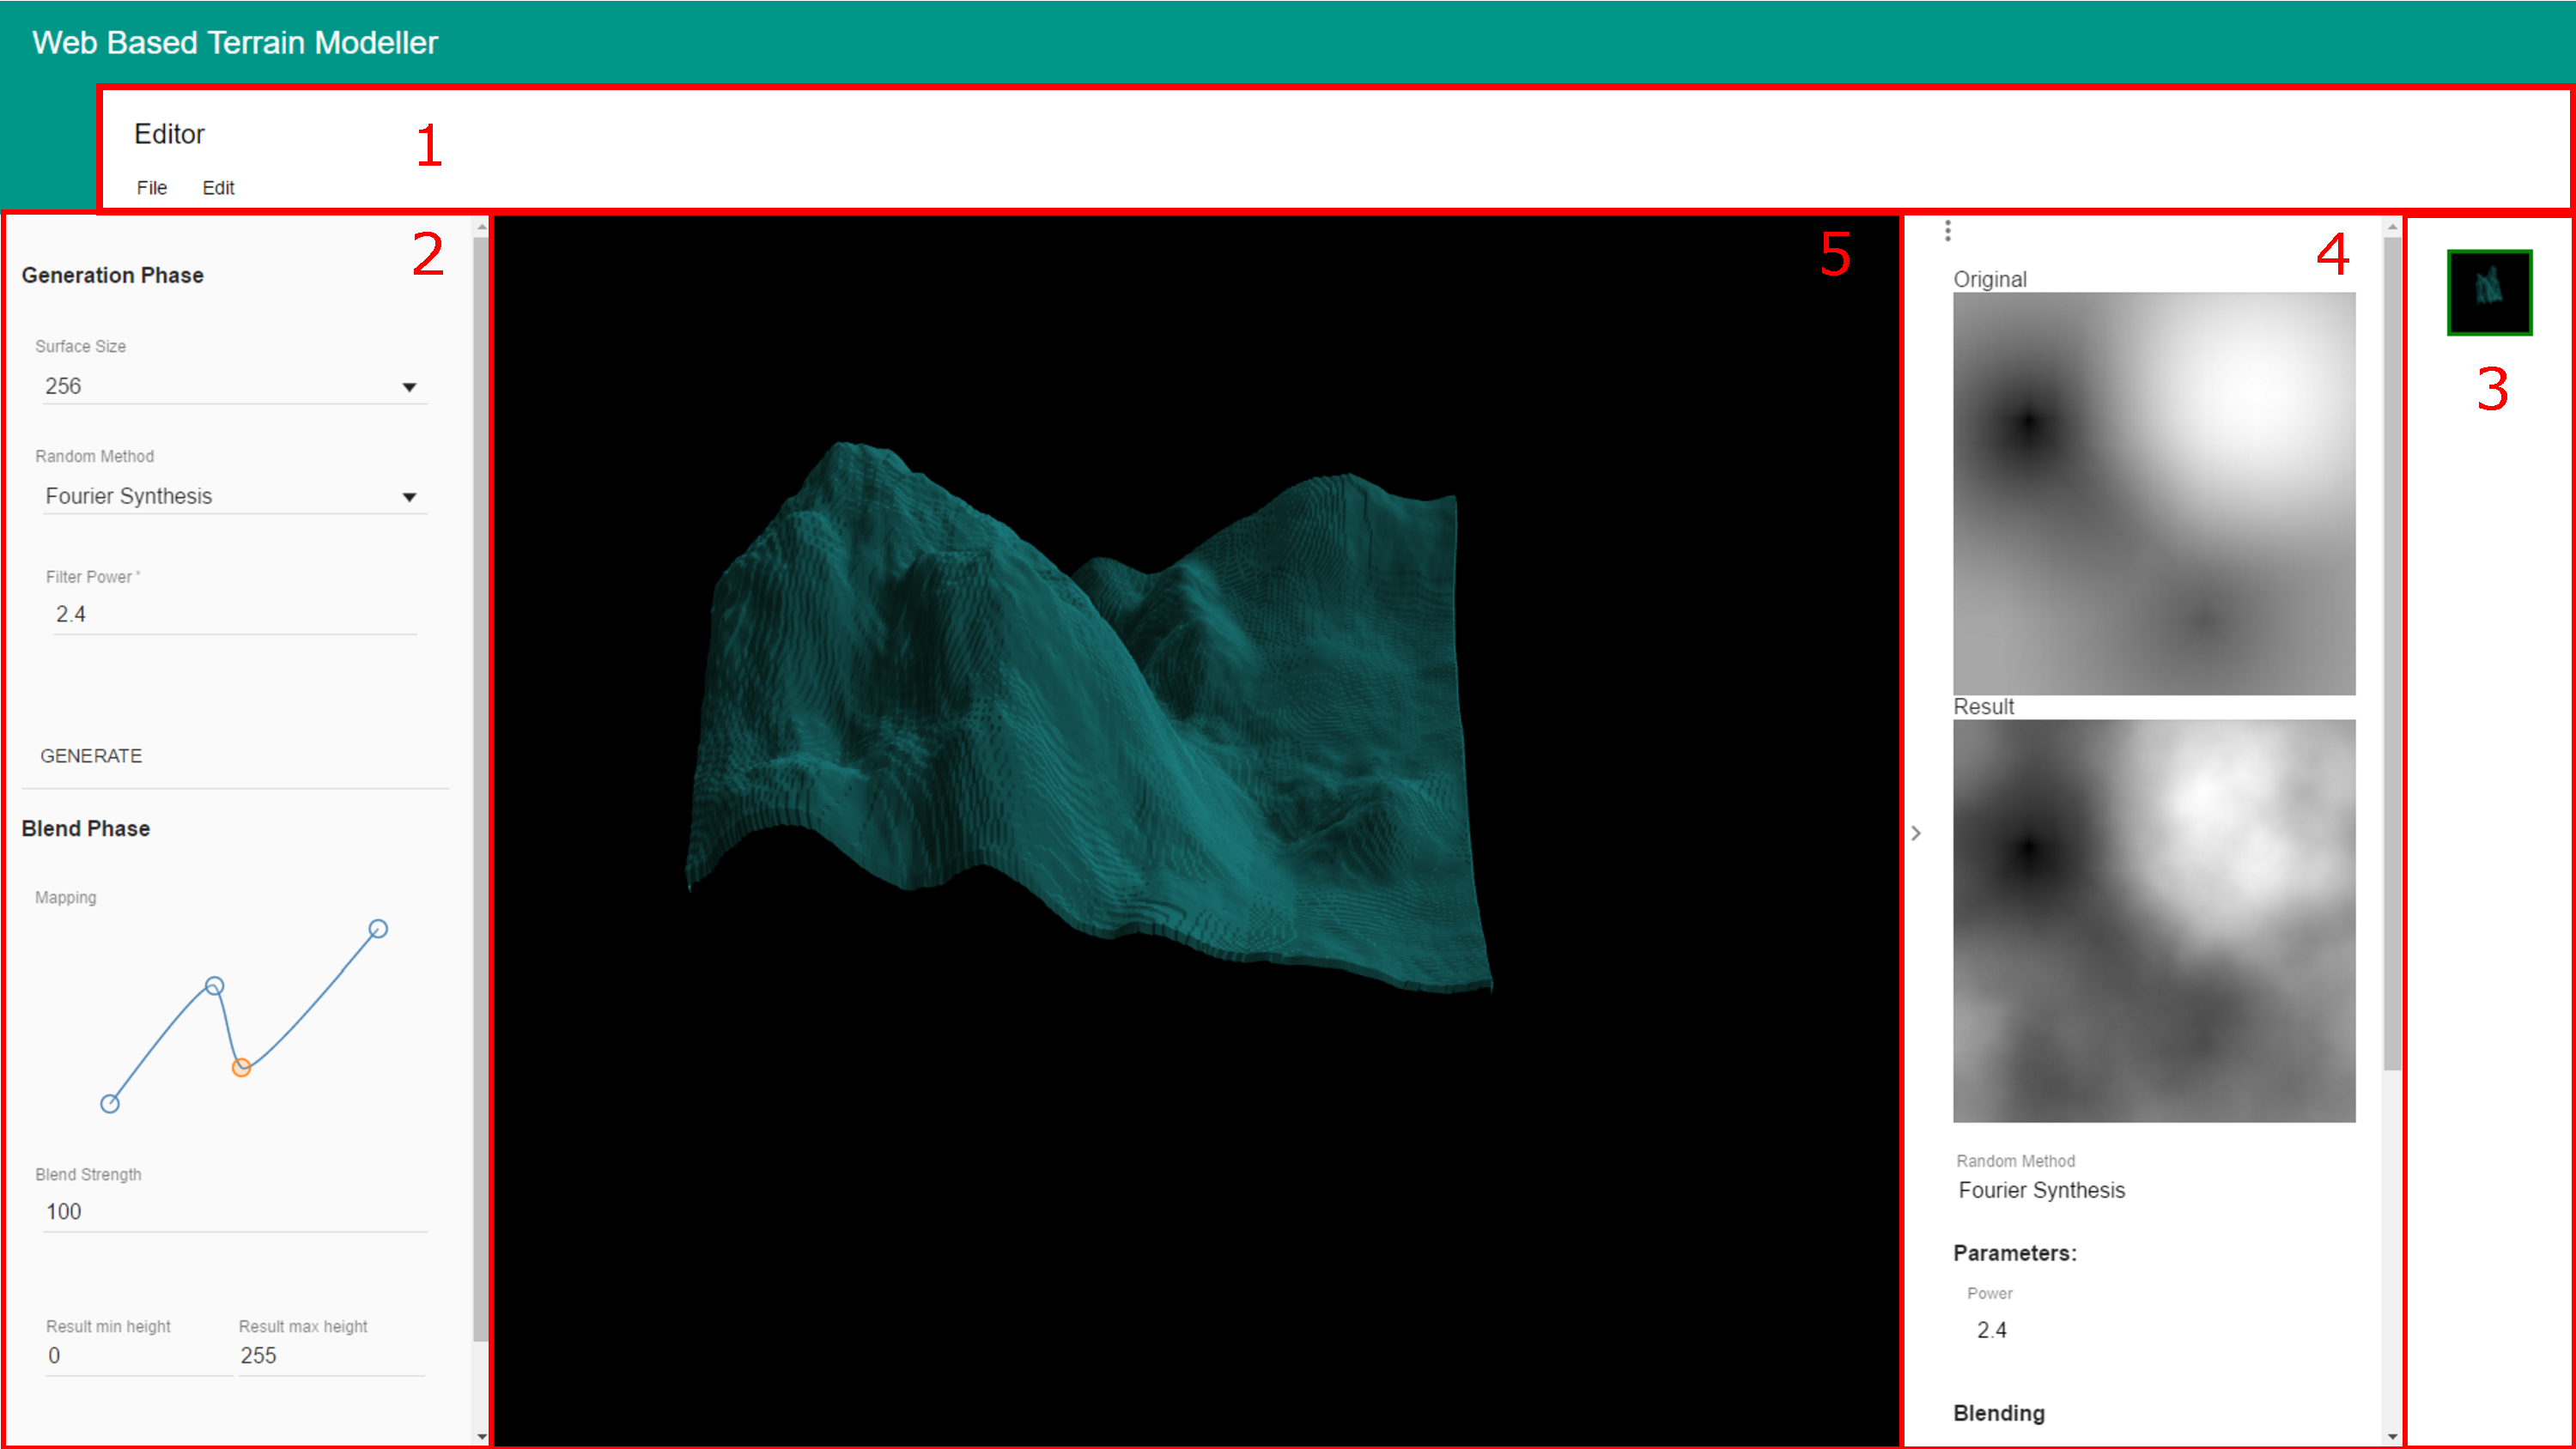
\includegraphics[width=0.95\linewidth]{images/screenshots/editorWithBoxes.pdf}
      	\caption{Editor Page}
      	\label{fig:editor_page}
      \end{figure}
      
      \begin{notes}
      	\item Explain each panel in detail or leave it only for user manual ???
      \end{notes}
    
    \subsection {Input and Output Formats}
    
      In order to allow the user to load and save his terrains the application implements an import and export feature. The user can either import a Grayscale PNG image, which will be set as the base surface, or import a previously exported Zip file, which will add an entry to the history list and render the result contained in the file. In terms of export formats the user can: obtain: a 4-channel 8-bit per channel PNG containing the height map of the result; a Zip file that can be later imported; and a Grayscale 1-channel 16-bit per channel PNG image of the result height map, which can be import as a landscape in Unreal Engine 4.

  \section {Physical Architecture} %CC Deployment View
    
    The system was developed as a client-side single page web application and thus all the server-side content is static. Given this properties the application works as a static web site and has a simple deployment architecture which consists on a HTTP web server and a web browser, as shown in Figure \ref{fig:deployment_diagram}.
    
    \begin{figure}[h!]
    	\begin{center}
    		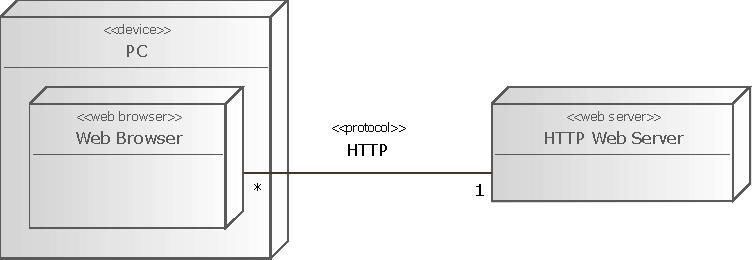
\includegraphics[width=0.9\textwidth]{images/diagrams/deployment.pdf}
    	\end{center}
    	\caption{Deployment Diagram}
    	\label{fig:deployment_diagram}
    \end{figure}
    
  \section {Implementation Architecture} %CC Implementation View
    
    The application is composed by three submodules (Figure \ref{fig:component_diagram}). The \textit{components} submodule is responsible for configuring the page routing and, as such, contains, as submodules, the editor and the benchmarks pages. The \textit{common} module contains services and directives that are generic to the application. The \textit{imgproc} module contains the image processing utilities.
    
    \begin{figure}[H]
      \begin{center}
      	 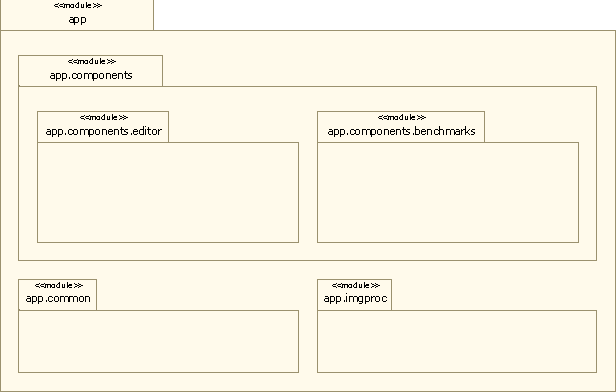
\includegraphics[width=0.9\textwidth]{images/diagrams/component.pdf}
      \end{center}
      \caption{Component Diagram}
      \label{fig:component_diagram}
    \end{figure}


    \subsection {Technologies}    
      
      Given the web-based requirement the application needed to be in Javascript. For convenience the Babel transpiler was used so that the development could be done in ECMAScript 6, which is a newer standard of Javascript. Additionally, to simplify the management of the required dependencies, JSPM and System.js were used, which, integrating with Babel, enable better support for ECMAScript 6 modules. 
      
      To aid the development of the application, Angular.js was used. This framework implements the MVC pattern, which was used to better modularize the source code.
      
      The terrain viewer was implemented using three.js, which is a 3D rendering Javascript library that allows the developer to create 3D Scenes in a straight forward way. 
      
      In order to parallelize some operations, WebGL 2.0 was used. This implementation will be detailed in section \ref{sec:software:process:gpu}
    
  \section {Logical View} %CC Logical View
  
	  The logical architecture of the developed application was influenced by the usage of Angular.js. Due to this in Figure \ref{fig:class_diagram}, where the UML class diagram for the application is shown, two prototypes are attributed to the classes: controller and service; the controller classes are responsible by the dynamic behaviour of the element to which they are attributed; the service classes are lazily instantiated singletons that are injected in the application in the required modules.
    
      \begin{figure}[H]
    	\begin{center}
    	  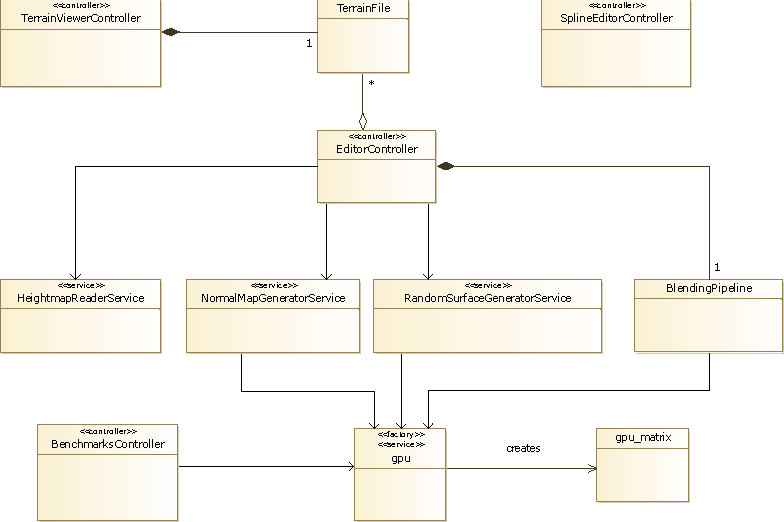
\includegraphics[width=\textwidth]{images/diagrams/class.pdf}
    	\end{center}
    	\caption{Class Diagram}
    	\label{fig:class_diagram}
      \end{figure}
    
  \section {Process View}
    
    \subsection {GPU Computation Framework} \label{sec:software:process:gpu} %CC Process View
    
      In order to optimize some operations performed by the application a GPU computation framework was implemented. This framework uses WebGL 2 to perform pixel-wise operations on images. WebGL 2 is a 3D rendering API for the web derived from OpenGL ES 3.0, which features a programmable rendering pipeline that gives the developer the ability to manipulate the rendering data in two different stages: the vertex stage and the fragment stage. The vertex stage executes the vertex shader using as input the vertex data and it outputs the final vertex position as a 4-component floating-point vector in homogeneous coordinates $(x, y, z, w)$. In the fragment stage the fragment shader is executed once per fragment and it's output depends on the active render target, which can be either the HTML canvas or a texture. When the render target is the HTML canvas the output is 4-component floating-point vector that represents the color of the fragment. When the render target is a texture the output depends on the texture format. For a texture to be a render target it's format needs to be \textit{color-renderable} and, in WebGL 1, as in OpenGL ES 2, only 3 or 4 component integer textures are \textit{color-renderable}. This limitation is surpassed in WebGL 2 and in OpenGL ES 3, where, with the \textit{EXT\_color\_buffer\_float} extension, floating-point textures with 1, 2, 3 or 4 components are considered \textit{color-renderable}.
      
      In order to use WebGL for computations the framework uses a texture as the render target and renders a square on a viewport of the same size as the texture, resulting in a 1:1 fragment to pixel mapping, and uses a specific fragment shader depending on the algorithm that is being executed. 
      
      \subsubsection{Implementation Details}
      
        To implement this framework two classes were created: the gpu class and the gpu\_matrix class (Figure \ref{fig:class_diagram}). The gpu class works as an Angular.js service which is injected wherever it is needed. At the same time this class is also factory for gpu\_matrix class instances, as the latter need an initialized gpu instance to be created, this is noted in the class diagram by the usage of the \textit{factory} prototype and the \textit{creates} relation between the two classes.
        
        The gpu\_matrix class represents a matrix that was uploaded to the GPU. Due to restrictions imposed by WebGL the textures dimensions need to be powers of 2 and their format is limited to 1, 2 or 4 components per pixel of 8 bits unsigned integer, 32 bits signed integer or 32 bits floating-point. This class handles the allocation and relocation of the textures and framebuffers, as well as, the upload and download of the matrix from a to the GPU device.
      
	  \subsubsection{Implemented algorithms}
	  
	    The implemented algorithms can be divided in 3 categories:
	    \begin{itemize}
	      \item Fast Fourier Transform
	      \item Element-wise Operations
	      \item Matrix Normalization
	    \end{itemize}
	    
	    The Fast Fourier Transform was implemented using the radix-2 Stockham FFT algorithm used in \cite{Lloyd2008}. This algorithm avoids the bit reversal phase of the FFT by reordering the dataflow and, consequently, cannot be performed in-place, which is not a problem for this implementation taking into account that textures in WebGL cannot be read from and written to at the same time. Additionally, as noted in \cite{Lloyd2008}, in order to compute a 2D FFT, the matrix is usually transposed to optimize the traversal of an array stored linearly in memory. This issue is also surpassed as, on a GPU, textures are swizzle, thus, no transposes are performed. 
	    To implement the Inverse Fast Fourier Transform the FFT implementation was used with the real and imaginary parts swapped as shown in \cite[p.450]{Lyons2004}.
	    
	    The element-wise operations implemented are addition, subtraction, multiplication and division. There are two version of this operations: the binary version, where two matrices are combined using the given operator, and the immediate version, where the operator is applied to matrix and to a given value. Additionally some image processing algorithms were implemented: two frequency domain filters: the gaussian blur and the $f^{-\beta}$, that were implemented by multiplying the fourier transform of the matrix by the fourier transform of the filter, which was computed using the analytical formulas; and a spatial domain sobel filter, both in x and y, which was implemented by performing a pixel-wise convolution of the matrix.
	    
	    In order to implement matrix normalization the process was divided in two phases. The first phase consists in finding the minimum and the maximum value of the matrix. The second is the element-wise execution of equation \ref{eq:software:gpu:norm}. To implement the first phase in parallel a reduction method was used. This method consists in first reducing each row to it's minimum and maximum, resulting in a vector of two values, and then reducing the resultant vector two the global minimum and maximum of the matrix.
	    
	    \begin{equation} \label{eq:software:gpu:norm}
		  M_{Normalized}(x, y) = \frac{M(x, y) - minimum_M}{maximum_M - minimum_M}
	    \end{equation}
	    \myequation{Normalization Operation}
	    
    \subsection {Blending Process Pipeline} %CC Process View
      
      In order to improve the application's performance a pipeline for the blending process was created. This pipeline saves the intermediate matrices of the blending process and reuses them when a parameter changes. This pipeline is illustrated in the activity diagram shown in Figure \ref{fig:activity_blending_process}, where the initial nodes represent the starting point when the associated parameter is modified. When this process reaches the final node a callback is invoked to trigger an update in the user interface.
      
      \begin{figure}[H]
      	\begin{center}
      	  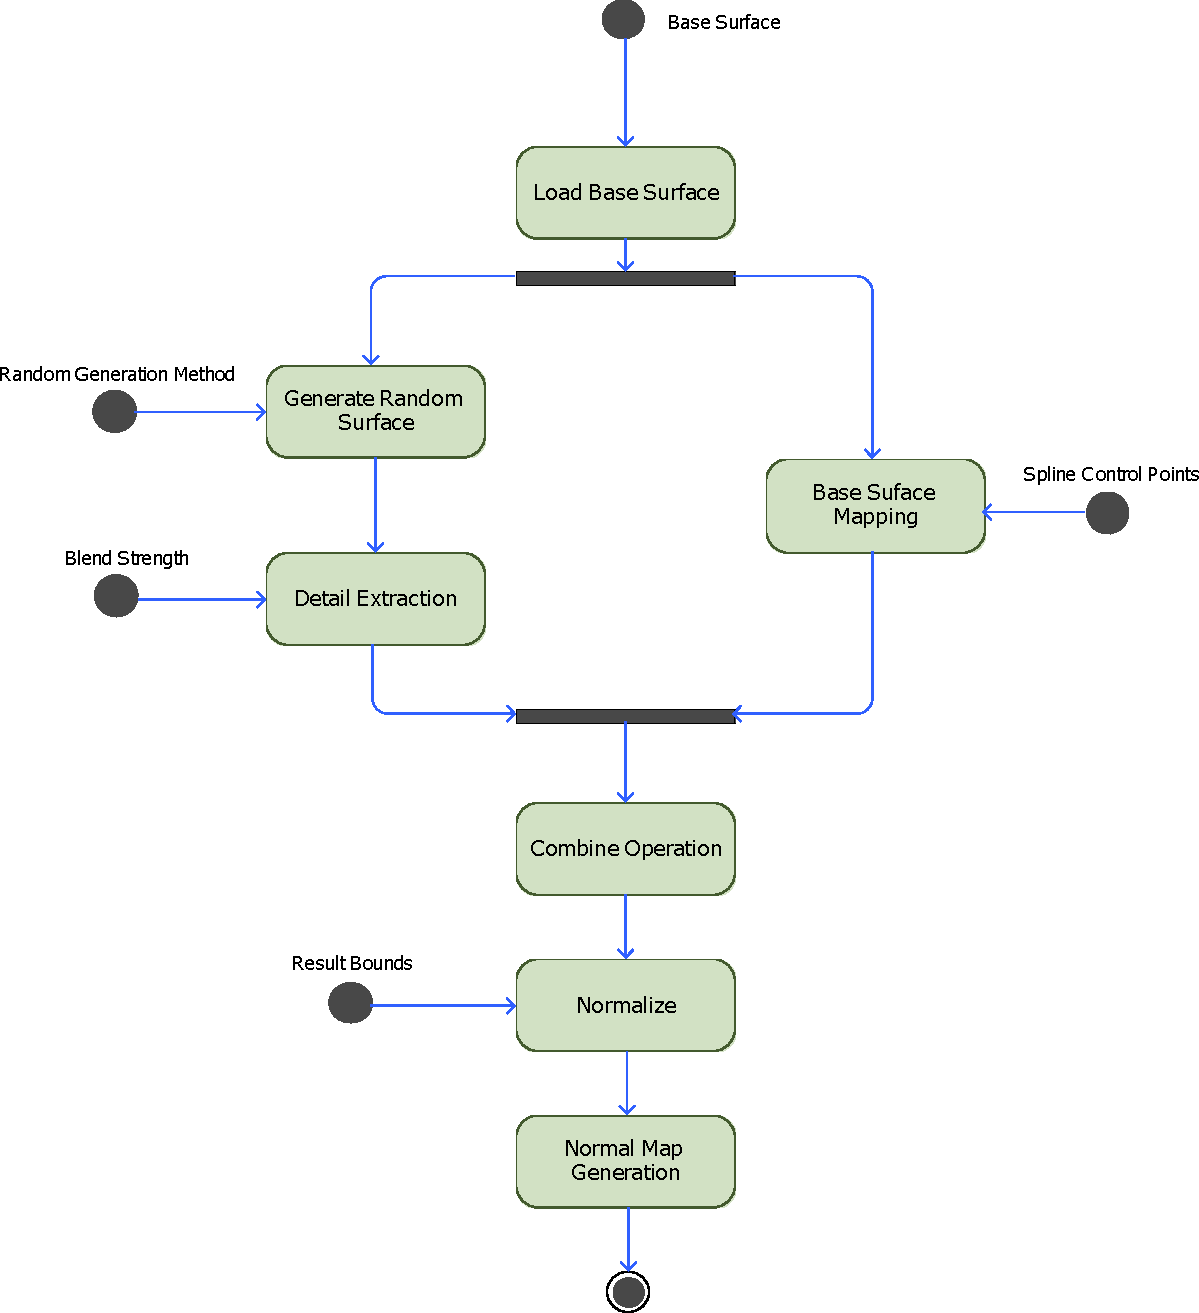
\includegraphics[width=\textwidth]{images/diagrams/blending_process.pdf}
      	\end{center}
        \caption{Activity diagram for the blending process}
        \label{fig:activity_blending_process}
      \end{figure} 